\documentclass{article}
\usepackage[utf8]{inputenc}
\usepackage{amsmath, amssymb, amsthm}
\usepackage[margin=1in]{geometry}
\usepackage{graphicx}  % For including images
\usepackage{listings}  % For including code
\usepackage{xcolor}  % For code highlighting
\usepackage{subcaption}  % For subfigures
\usepackage{hyperref}
\usepackage{tikz}
\usepackage{pdfpages}
\usetikzlibrary{positioning}

% Define theorem environments
\newtheorem{theorem}{Theorem}
\newtheorem{lemma}{Lemma}
\newtheorem{definition}{Definition}
\newtheorem{corollary}{Corollary}
% Define custom solution environment
\newenvironment{solution}{\noindent\textbf{Solution:} }{\qed}
% Code listing style
\lstset{
    language=Python,
    basicstyle=\ttfamily\footnotesize,
    keywordstyle=\color{blue},
    commentstyle=\color{gray},
    stringstyle=\color{red},
    breaklines=true,
    numbers=left,
    numberstyle=\tiny\color{gray},
    frame=single
}
\usetikzlibrary{positioning, shapes, arrows.meta}

\title{ECE-GY 7143 Introduction to Deep Learning \\ \Large Homework 2}
\author{Ali Hamza (ah7072)}
\date{\today}

\begin{document}
\maketitle
\newpage
\section*{Question 1}
\begin{figure}[ht]
    \centering
    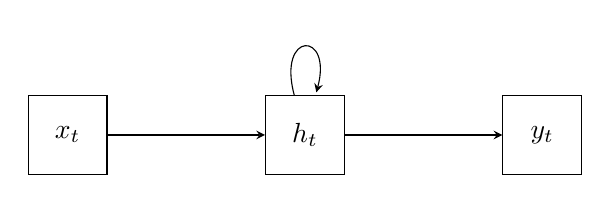
\begin{tikzpicture}[>=stealth, node distance=2cm, auto]
    % Input node
    \node[draw, rectangle, minimum width=1cm, minimum height=1cm] (xt) {$x_t$};
    \node[draw, rectangle, right=of xt, minimum width=1cm, minimum height=1cm] (ht) {$h_t$};
    \node[draw, rectangle, right=of ht, minimum width=1cm, minimum height=1cm] (yt) {$y_t$};
    % Connections: input to hidden layer
    \draw[->] (xt) -- (ht);
    % Connections: hidden layer to output 
    \draw[->] (ht) -- (yt);
    % Connections: hidden layer to hidden layer (looping arrow)
    \draw[->] (ht) edge[loop above] node {} (ht);
\end{tikzpicture}
    \caption{RNN Architecture}
    \label{rnn_architecture}
\end{figure}
\noindent Given the RNN in Figure \ref{rnn_architecture}, the following equations describe the forward pass of the RNN:
\begin{align*}
    h_t &= x_t + W_h h_{t-1}\\
    y_t &= \text{Sigmoid}(W_y h_t)
\end{align*}
where $h_t$ is the hidden state at time $t$, $x_t$ is the input at time $t$ and $y_t$ is the output at time $t$. The weights are $W_h = -1$ and $W_y = 1000$. 
Assuming $h_0 = 0$. The RNN is unrolled for $T$ time steps as follows:
\begin{align*}
    h_1 &= x_1\\
    h_2 &= x_2 - h_1 = x_2 - x_1\\
    h_3 &= x_3 - h_2 = x_3 - (x_2 - x_1) = x_3 - x_2 + x_1\\
    h_4 &= x_4 - h_3 = x_4 - (x_3 - x_2 + x_1) = x_4 - x_3 + x_2 - x_1\\
    \vdots \\
    h_T &= x_T - h_{T-1} = x_T - x_{T-1} + x_{T-2} - \ldots + (-1)^{T-1} x_1
\end{align*}
Then for $T=1000$, $h_T$ can be expressed as:
\begin{align*}
    h_{1000} &= x_{1000} - x_{999} + x_{998} - \ldots + (-1)^{999} x_1
\end{align*}
The output $y_T$ is given by:
\begin{align*}
    y_T &= \text{Sigmoid}(W_y h_T)\\
    &= \text{Sigmoid}(1000 \cdot h_{1000})
\end{align*}
Given that $\text{Sigmoid}$ function is defined as:
\begin{align*}
    \text{Sigmoid}(x) &= \frac{1}{1 + e^{-x}}
\end{align*}
We know that $\lim_{x \to \infty} \text{Sigmoid}(x) = 1$ and $\lim_{x \to -\infty} \text{Sigmoid}(x) = 0$. Therefore, we can analyze the output $y_T$ based on the value of $h_{1000}$:
\begin{align*}
    y_T &= \text{Sigmoid}(1000 \cdot h_{1000})\\
    &= \begin{cases}
        1 & \text{if } \lim_{h_{1000} \to \infty}\\
        0 & \text{if } \lim_{h_{1000} \to -\infty}\\
        0.5 & \text{if } h_{1000} = 0
    \end{cases}
\end{align*}

Thus, the output $y_T$ can be interpreted as a binary classification of $x_t$ based on the alternating sum of the inputs. If the sum is positive, the output is close to 1, and if the sum is negative, the output is close to 0. If the sum is zero, the output is 0.5.

\section*{Question 2}
Let $X \in \mathbb{R}^{T \times d_{model}}$ be the input embeddings for a sequence of length $T$.
Let $W_Q, W_K, W_V$ be learned weight matrices.
The Query, Key, and Value matrices are $Q = XW_Q \in \mathbb{R}^{T \times d_k}$, $K = XW_K \in \mathbb{R}^{T \times d_k}$, $V = XW_V \in \mathbb{R}^{T \times d_v}$.
Computing Q, K, V takes $O(T d_{model} d_k + T d_{model} d_v) = O(T)$ time, assuming fixed dimensions $d_{model}, d_k, d_v$.

\subsection*{Standard Self-Attention: $O(T^2)$}
Standard attention is computed as:
\[
Attention(Q, K, V) = \text{softmax}\left(\frac{QK^T}{\sqrt{d_k}}\right) V
\]
The computational bottleneck stems from the $QK^T$ operation:
\begin{enumerate}
    \item \textbf{Score Matrix $A = QK^T$}: Calculation involves multiplying a $(T \times d_k)$ matrix by a $(d_k \times T)$ matrix.
    \begin{itemize}
        \item Output Size: $T \times T$.
        \item Complexity: $O(T \cdot d_k \cdot T) = O(T^2 d_k)$. Since $d_k$ is fixed, this is $\boldsymbol{O(T^2)}$.
    \end{itemize}
    \item \textbf{Subsequent Operations}: Applying scaling, softmax, and multiplication by $V$ ($W V$) involve operations on the $T \times T$ score or weight matrix.
    \begin{itemize}
        \item Softmax Complexity: $O(T^2)$.
        \item $WV$ Complexity: Multiplication of $(T \times T)$ by $(T \times d_v)$ is $O(T^2 d_v) = \boldsymbol{O(T^2)}$.
    \end{itemize}
\end{enumerate}
The explicit computation and manipulation of the $T \times T$ attention matrix lead to an overall $\boldsymbol{O(T^2)}$ complexity.

\subsection*{Linear Self-Attention: $O(T)$}
This variant replaces the softmax normalization. Instead of $\text{softmax}(A)_{ij} = \frac{\exp(A_{ij})}{\sum_k \exp(A_{ik})}$, a linear normalization is used, effectively computing $\tilde{A}_{ij} = \frac{A_{ij}}{\sum_k A_{ik}}$ (assuming $A_{ik} > 0$). The crucial optimization comes from changing the order of operations using matrix associativity, avoiding the explicit computation of $A = QK^T$.\\

\noindent Instead of calculating $(QK^T)V$, we compute $Q(K^T V)$:
\begin{enumerate}
    \item \textbf{Compute $K^T V$}: Multiply $(d_k \times T)$ matrix $K^T$ by $(T \times d_v)$ matrix $V$.
    \begin{itemize}
        \item Output Size: $d_k \times d_v$ (independent of $T$).
        \item Complexity: $O(d_k \cdot T \cdot d_v) = \boldsymbol{O(T)}$. Let $Temp = K^T V$.
    \end{itemize}
    \item \textbf{Compute $Q (K^T V)$}: Multiply $(T \times d_k)$ matrix $Q$ by $(d_k \times d_v)$ matrix $Temp$.
    \begin{itemize}
        \item Output Size: $T \times d_v$.
        \item Complexity: $O(T \cdot d_k \cdot d_v) = \boldsymbol{O(T)}$. This gives the unnormalized output, let's call it $O_{unnorm}$.
    \end{itemize}
    \item \textbf{Compute Normalization Factors}: The denominator for row $i$ is $\sum_k (QK^T)_{ik} = Q_i (\sum_k K_k^T)$. We need this sum for each $Q_i$.
    \begin{itemize}
        \item Calculate $K_{sum}^T = \sum_{k=1}^T K_k^T \in \mathbb{R}^{d_k \times 1}$. Requires summing $T$ vectors of size $d_k$. Complexity $O(T d_k) = O(T)$.
        \item Calculate normalization vector $D = Q K_{sum}^T \in \mathbb{R}^{T \times 1}$. Multiply $(T \times d_k)$ by $(d_k \times 1)$. Complexity $O(T d_k) = \boldsymbol{O(T)}$. $D_i$ contains the sum for row $i$.
    \end{itemize}
    \item \textbf{Apply Normalization}: Divide each element $(O_{unnorm})_{ij}$ by $D_i$.
    \begin{itemize}
        \item Element-wise operation on a $T \times d_v$ matrix.
        \item Complexity: $O(T d_v) = \boldsymbol{O(T)}$.
    \end{itemize}
\end{enumerate}
By rearranging the computation to $Q(K^T V)$ and calculating the linear normalization factor efficiently, we avoid forming the $T \times T$ matrix. All steps are linear in $T$, resulting in an overall complexity of $\boldsymbol{O(T)}$.

\section*{Question 3}

The goal was to implement and evaluate Vision Transformer (ViT) models on the FashionMNIST dataset by experimenting with different architectural configurations, specifically varying the number of transformer layers (4–8) and attention heads (2–4)

\subsection*{Data Preparation}
The FashionMNIST dataset was loaded, normalized, and split (80\% train, 20\% test). Data loaders were set up with a batch size of 64.

\subsection*{Model Architecture}
The ViT implementation includes:
\begin{itemize}
    \item \textbf{Patch Embeddings:}
    The \texttt{PatchEmbeddings} class splits the input image into fixed-size patches (e.g., 4×4 pixels). It uses a convolutional layer with a kernel size and stride equal to the patch size. This layer not only extracts non-overlapping patches but also projects each patch into a higher-dimensional latent space (the embedding space). The resulting output is a sequence of patch embeddings.
    \item \textbf{[CLS] Token \& Positional Embeddings:}  
      In the \texttt{Embeddings} class, a learnable \texttt{[CLS]} token is prepended to the sequence of patch embeddings. This token is designed to capture the global information needed for classification. Additionally, positional embeddings are added to the sequence, which provide the model with information about the spatial arrangement of the patches. This is crucial since transformers are permutation-invariant and require positional cues to understand the order of the patches.
      
    \item \textbf{Transformer Encoder:}  
        The encoder is constructed as a stack of transformer blocks (implemented in the \texttt{Encoder} class). Each block (defined in the \texttt{Block} class) consists of two main components:
        \begin{enumerate}
            \item \textbf{Multi-Head Self-Attention:}  
                    The \texttt{MultiHeadAttention} module aggregates information from all patches by computing attention scores across the entire sequence. It first splits the input into multiple heads (using the \texttt{AttentionHead} class) to capture different aspects of the relationships among patches. The outputs of these heads are then concatenated and projected back to the original embedding dimension.
            \item \textbf{Feed-Forward Network (MLP):}  
                    The \texttt{MLP} module applies two linear transformations with a GELU activation in between. This network further processes the output from the self-attention layer, and a dropout is applied to prevent overfitting.
        \end{enumerate}
        Both components in each block are wrapped with layer normalization and are connected via skip (residual) connections. This design helps stabilize training and allows the model to learn deep representations.
        
    \item \textbf{Classification Head:}  
        After passing through the transformer encoder, only the output corresponding to the \texttt{[CLS]} token is used for classification. The \texttt{ViT} class ends with a simple linear layer that maps the \texttt{[CLS]} token representation to the desired number of class logits.
\end{itemize}

\subsection*{Training Setup}
Cross-entropy loss was used along with the Adam optimizer (learning rate = 0.01) and a StepLR scheduler (halving the learning rate every 5 epochs). For each experiment, training loss and test accuracy were recorded. Each model was trained for 25 epochs

\subsection*{Experiment Range \& Evaluation}
Experiments were run for each combination all conbinations of layers (4 to 8) and heads (2 to 4). Train loss and test accuracy were tracked over 25 epochs and confusion matrices were computed on the test set to analyze misclassifications. 

\newpage
\subsection*{Results}

\begin{table}[ht]
    \centering
    \begin{tabular}{|c|c|c|c|}
        \hline
        \textbf{Layers} & \textbf{Heads} & \textbf{Train Loss} & \textbf{Test Accuracy} \\
        \hline
        4 & 2 & 0.0690 & 87.86\% \\
        4 & 3 & 0.0443 & 88.02\% \\
        4 & 4 & 0.0357 & 87.73\% \\
        \hline
        5 & 2 & 0.0680 & 87.83\% \\
        5 & 3 & 0.0339 & 88.89\% \\
        5 & 4 & 0.0269 & 88.32\% \\
        \hline
        6 & 2 & 0.0378 & 87.65\% \\
        6 & 3 & 0.0380 & 87.54\% \\
        6 & 4 & 0.0323 & 88.08\% \\
        \hline
        7 & 2 & 0.0787 & 88.73\% \\
        7 & 3 & 0.0255 & 88.73\% \\
        7 & 4 & 0.0229 & 88.52\% \\
        \hline
        8 & 2 & 0.0342 & 87.84\% \\
        8 & 3 & 0.0342 & 87.84\% \\
        8 & 4 & 0.0200 & 88.46\% \\
        \hline
    \end{tabular}
    \caption{Summary of Results for Different Model Configurations}
    \label{tab:results}
\end{table}

\begin{figure}[ht]
    \centering
    \begin{minipage}{0.48\textwidth}
      \centering
      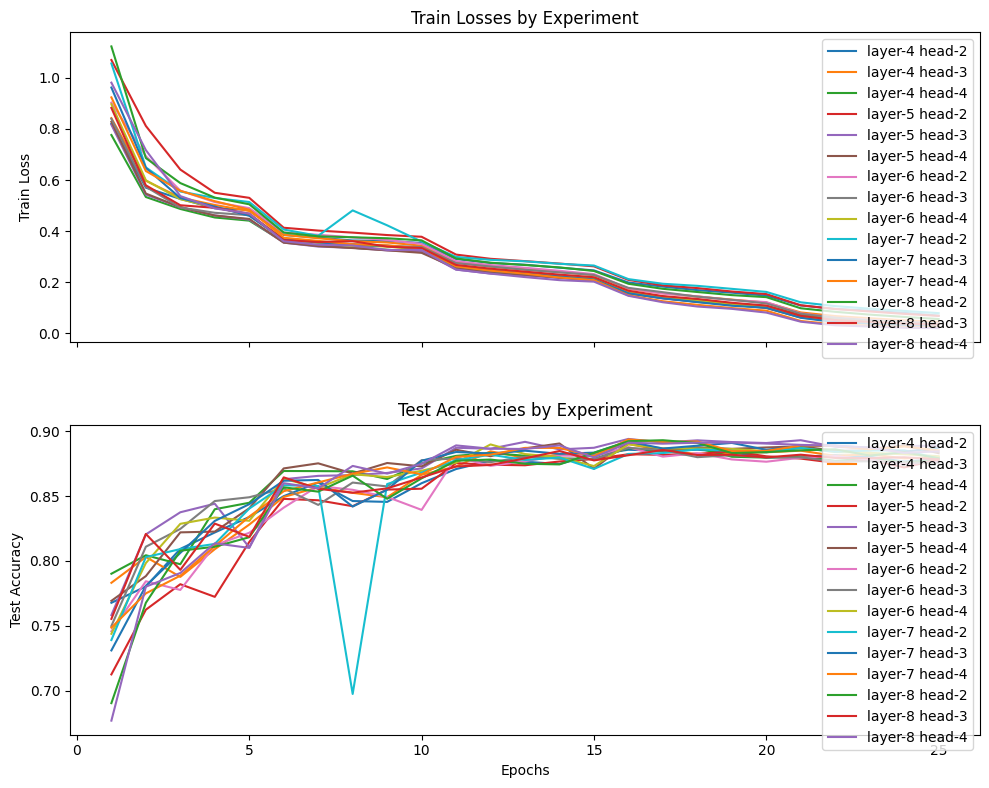
\includegraphics[width=\textwidth]{losses.png}
      \caption{Training Losses and Test Accuracies for all Experiments}
      \label{fig:train_test_loss}
    \end{minipage}\hfill
    \begin{minipage}{0.48\textwidth}
      \centering
      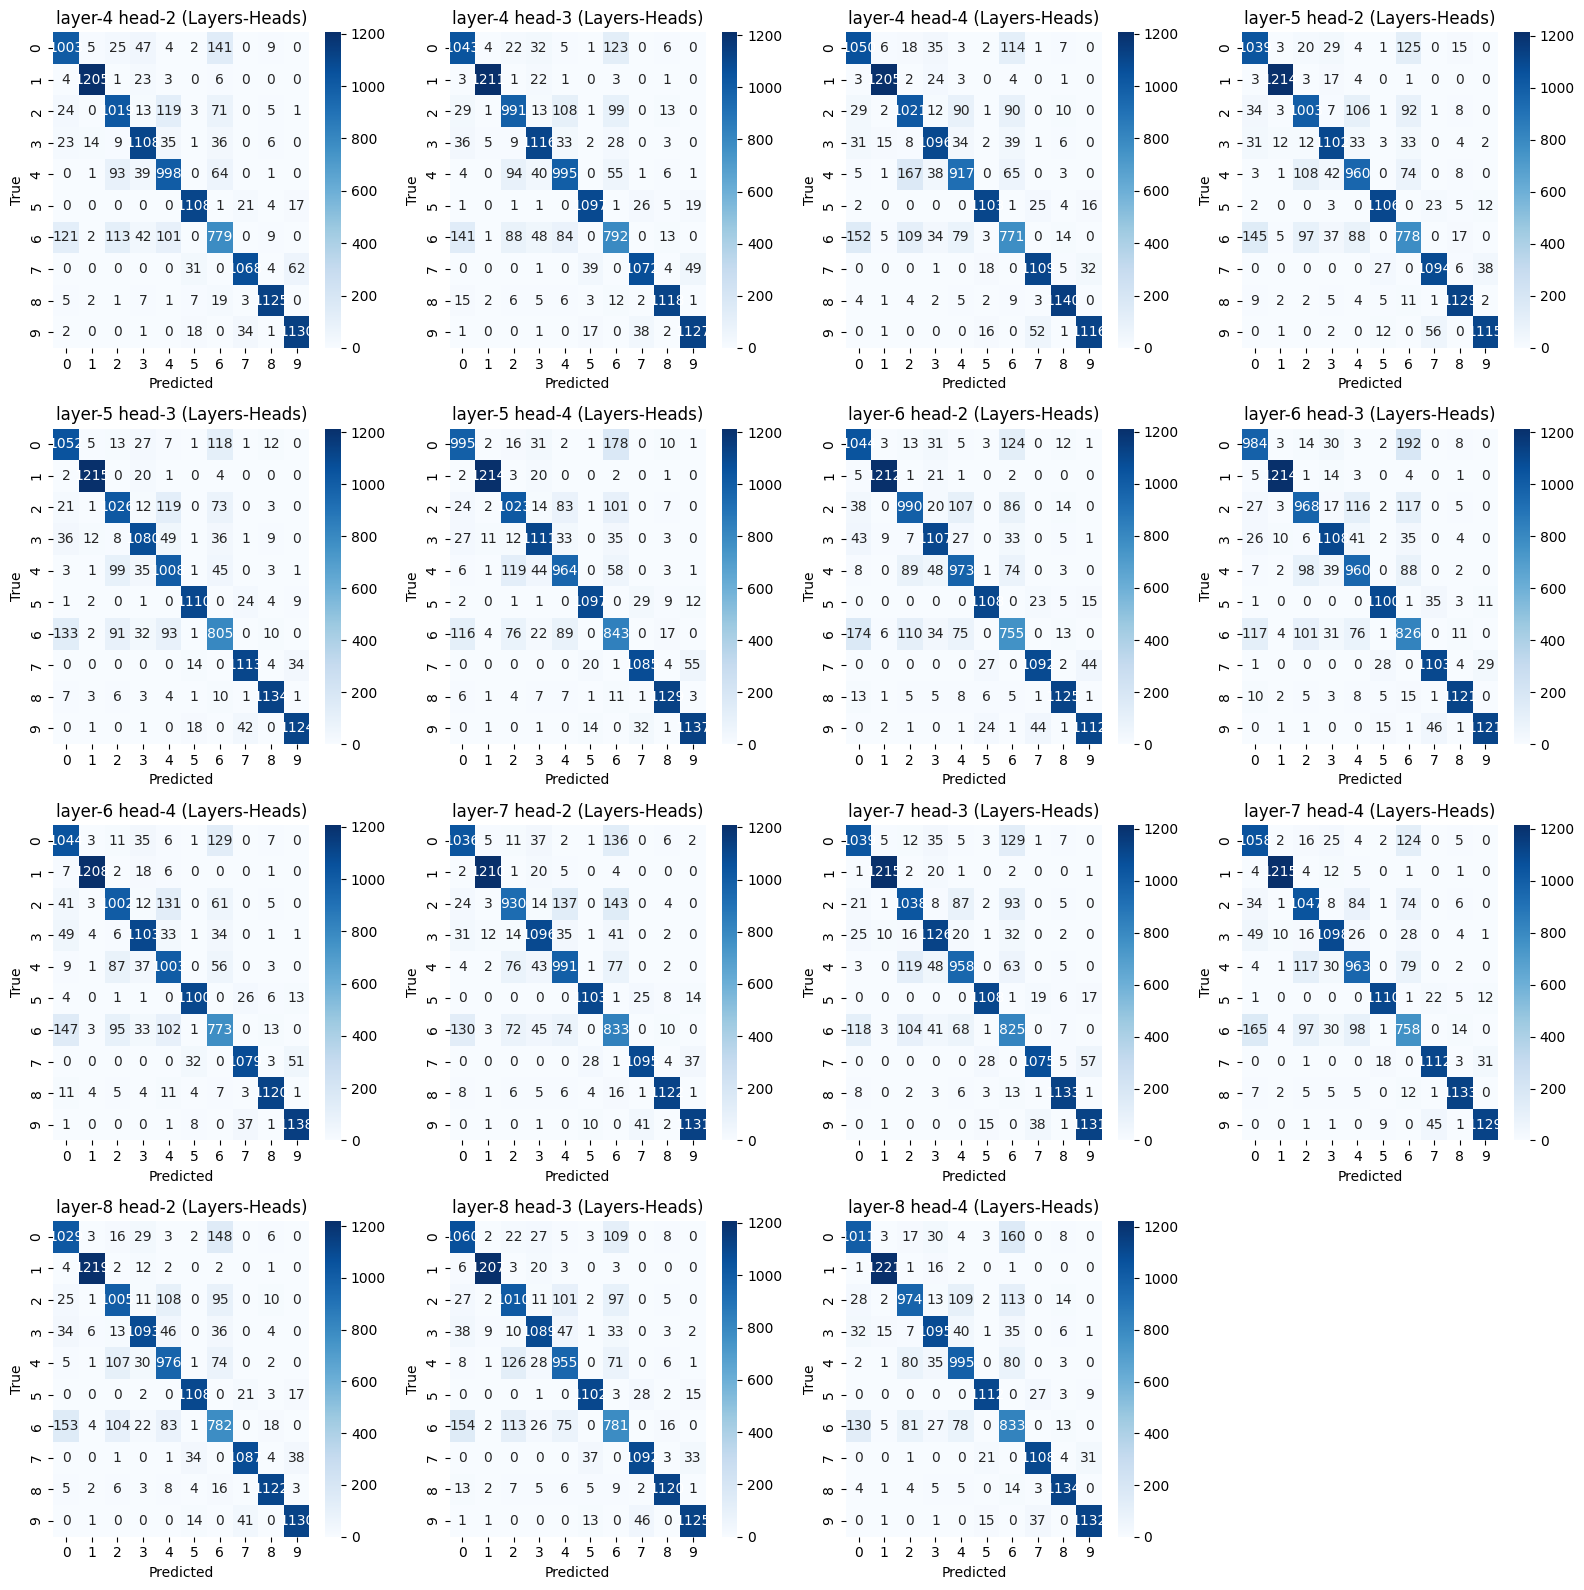
\includegraphics[width=\textwidth]{conf_mat.png}
      \caption{Confusion Matrices for all Model Configurations}
      \label{fig:confusion_matrix}
    \end{minipage}
  \end{figure}


\subsection*{Discussion}
We observe that increasing the number of layers and attention heads for this dataset doesn't significantly improve performance. The model with 5 layers and 4 heads achieved the best test accuracy of 88.89\%. The confusion matrices indicate that all model struggle with classifying the digit 6 but perform well on other classes.  

\includepdf[pages=-]{hw2_q3.pdf}

\section*{Question 4}
\includepdf[pages=-]{hw2_q4.pdf}

\section*{References}
\begin{enumerate}
    \item \href{https://d2l.ai/chapter_recurrent-neural-networks/rnn.html}{Recurrent Neural Networks}
    \item \href{https://tintn.github.io/Implementing-Vision-Transformer-from-Scratch/}{Implementing Vision Transformer from Scratch}
    \item GPT o3-mini-high used for brainstorming, debugging, and report writing.
\end{enumerate}
\end{document}